% We are thrilled to announce the launch of the groundbreaking ByteBoost Cybertraining Program. ByteBoost is driven by the imperative to enhance researchers' proficiency and productivity when navigating cutting-edge, specialized computing technologies. We hope to empower researchers to make the best computing choices in the ever-changing landscape of computational technology. This initiative will focus on supporting researchers using the technologies of three NSF computing testbeds - Ookami, Neocortex and ACES.

% Program Objectives:
% Facilitate Seamless Research: Elevate the ease and productivity of researchers working with cutting-edge computing technology.
% Community Growth: Foster a well-informed community of computational researchers adept at handling the newest technologies and porting applications.
% Optimal Testbed Usage: Ensure the proper and efficient utilization of testbeds, a critical component in the recent surge of data-enabled science and engineering.
% Target Audience:
% Early career-researchers (graduate students, postdoctoral associates, and Assistant Professors) from all fields of computationally inclined research

% Submission Guidelines
% Submission must include the following
% CV (1 page) including the applicant's previous computing experiences, skills, and field of science
% Abstract (1 page) - Prospective participants are required to submit an abstract outlining the specific topic they intend to explore as a fundamental part of their application for consideration in this call for participation.
\noindent
\textbf{Foundations for Agent-based Evolution on Emerging HPC Accelerators.}
M.A. Moreno, \texttt{morenoma@umich.edu}

\section{Introduction}
Evolutionary processes underlie key questions in public health, medicine, and natural resources management.
In conjunction with benchtop experiments and observational studies, mathematical and computational models play a key role in our understanding of evolutionary processes underpinning critical problems like epidemiology, antibiotic resistance, cancer biology, and conservation biology.
Emerging massively parallel/distributed High-Performance Computing (HPC) hardware like the Cerebras Wafer-Scale Engine (WSE) and Graphcore Intelligence Processing Unit (IPU) platforms will provide a foothold for model-driven inquiry into key cross-scale research questions, such as major transitions in evolution (e.g., origins of multicellularity) and evo-epidemiological relationships between within-host infection dynamics and population-level transmission patterns.
However, foundational algorithms and supporting software (e.g., Cerebras Software Language [CSL], Poplar) necessary to harness these platforms for agent-based evolution simulations remain largely undeveloped.
Progress on these fronts will contribute to broader classes of agent-based model (ABM) simulation.

\section{Methods}

\begin{wrapfigure}{R}{2in}
% \begin{minipage}{3in}
\vspace{-3ex}
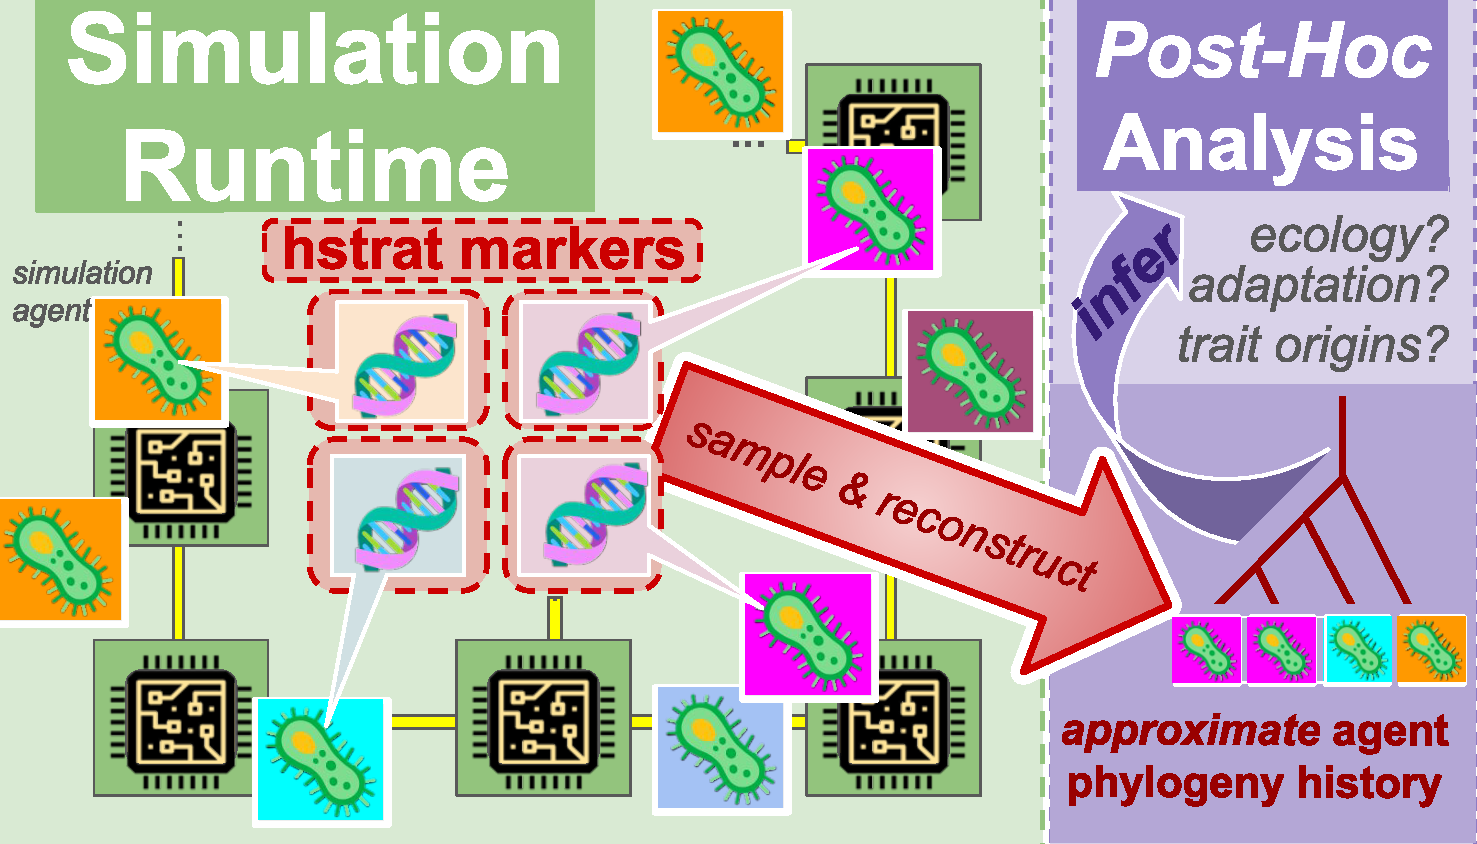
\includegraphics[width=2in]{img/runtime-posthoc-schematic.pdf}
% \end{minipage}%
% \begin{minipage}{2in}
\vspace{-5ex}
\caption{\footnotesize
Evolution simulation with reconstruction-based lineage analysis.}
\label{fig:runtime-posthoc-schematic}
\vspace{-2ex}
% \end{minipage}
\end{wrapfigure}


To succeed as a tool for scientific research, simulation must be sufficiently observable.
Within the  evolutionary simulations, the constitutes an important thing.
However, due to issues, direct tracking methods scale poorly to multiprocess contexts \cite{moreno2024analysis}. feasible particularly memory-constrained.

Proposed work builds on recently-introduced \textit{hereditary stratigraphy} (HStrat) methodology for extraction of evolutionary history from large-scale parallel and distributed evolutionary simulations \cite{moreno2022hstrat}.
Each genome in a population is marked with a special annotation akin to noncoding DNA (as small as 96 bits), inherited by each consecutive generation.
At the end of a simulation, these markers facilitate post-hoc analysis of evolutionary history (e.g., reconstructing phylogenetic history), shown in Figure 1.

In recent work, we have taken major strides towards this vision with the Cerebras SDK, phylogenetic reconstruction using hereditary stratigraphy techniques and managing a population using asynchronous agent migration between neighboring PEs.
\url{https://github.com/mmore500/wse-sketches}


\section{Proposed Work}

What conditions precipitate emergence/success of new viral strains?
In particular, how does the population size/infection intensity affect the rate at which strains emerge/sweep? \cite{markov2023evolution}.

Possible engineering questions scoped to a workshop environment include,
\begin{itemize}
\item How to efficiently perform long-distance migration?
One possibility is to impose an overlay of fixed long distance routes.
Another would be stochastic forwarding.
How best to take advantage of built-routing capabilities will benefit from instruction in the workshop.
This is important to be able to create more realistic population structures that deviate beyond simple grid connectivity.
\item How to sample population members on-the-fly?
The builtin memcpy operation provides a good way to do this at conclusion, but advanced techniques for asynchronous memcpy operations or otherwise.
\end{itemize}

\section{Broader Impacts}

The availability of modular, extendable software for agent-based evolution simulation on emerging HPC architectures will catalyze research.
Progress on this front
How to organize, test, and distribute CSL and Poplar modules, to directly create modules during the workshop that can be shared.
If there aren’t established protocols, the workshop environment would be a great place to discuss these issues.

I am excited to share what I learn at the workshop within my academic circles.
As a participant in the Schmidt AI in Science Postdoctoral Scholar program at University of Michigan, I regularly to lead.
I will be excited to share with my cohort of 10 peer scholars from domains across the natural sciences, with weekly seminar series focused on peer cross-pollination.

I hope to use this opportunity to build connections in HPC world, to SAY SOMETHING ABOUT CAREER AND CAREER STAGE.
I am currently preparing an ACCESS Innovative Projects Proposal and recently submitted a preproposal for the Dept. of Energy's EXPRESS 2024 FOA.
Foundations for extensive ongoing work pushing ABM into these directions in my own career.
Ultimately, I hope this workshop pwoposal will contribute to lay foundations for research in open—ended evolution (cite MODES) and in evolutionary epidemiology, among other topics. and lay foundations in my own career to continue to develop those foundations for the research community I work in.

% What is the structural relationship between individual-level phylogenies and species-level phylogenies?
% Do they respond in the same way to evolutionary conditions like selection pressure, ecology, and spatial structure?
